\documentclass[12pt]{article}
\usepackage{graphicx}
\usepackage{float}
\usepackage{xcolor}
\usepackage[margin=1in]{geometry}
\usepackage{amsmath}

\newcommand{\myvspace}{\vspace{4mm} \noindent}

\newcommand{\question}[1]{\vspace{10mm} \noindent {\bf #1)}~~}

\begin{document}
%\pagestyle{empty}

\begin{center}
\bf ASTR150 Exoplanet Lab
\end{center}

Some planets orbiting stars in other solar systems -- called {\bf exoplanets} -- appear to pass in front of their stars once per orbit. If you could use a super-powerful telescope that could ``zoom in'' far enough, you would be able to see the planet eclipse the star. We don't have telescopes powerful enough to do this, so instead we carefully measure the brightness of the host stars and detect the small decrease in brightness that occurs when the planet blocks out a fraction of the star light once per orbit.  We call these eclipses {\bf transit} events, and this is how the majority of planets have been discovered to date.
\begin{figure}[h!]
\centering
\includegraphics[scale=0.2]{plots/transit.eps}
%\vspace{-5mm}
%\caption{Notice the difference in the scale of the y-axis in each plot!}
\end{figure}

{\bf The amount of light that a planet blocks out, known as the transit depth} is related to how big the planet is. If the planet were the same size (had the same radius) as the star it would block out the star light completely when it passed in front, and if the planet were the size of a piece of dust it wouldn't block out much light at all. This means that we can measure the ratio of the radius of the planet to the radius of the star by measuring how much light is blocked out: 
\begin{equation}
\mathrm{Change~in~brightness} = \left( \frac{\mathrm{Radius~of~the~planet}}{\mathrm{Radius~of~the~star}} \right)^2 \label{eqn:depth}
\end{equation}
Now assume that we measured the brightness of a star that has the same mass and radius as the Sun and found the following transit events:
\pagebreak

\begin{figure}[h!]
\centering
{\bf Transit Detections} \\
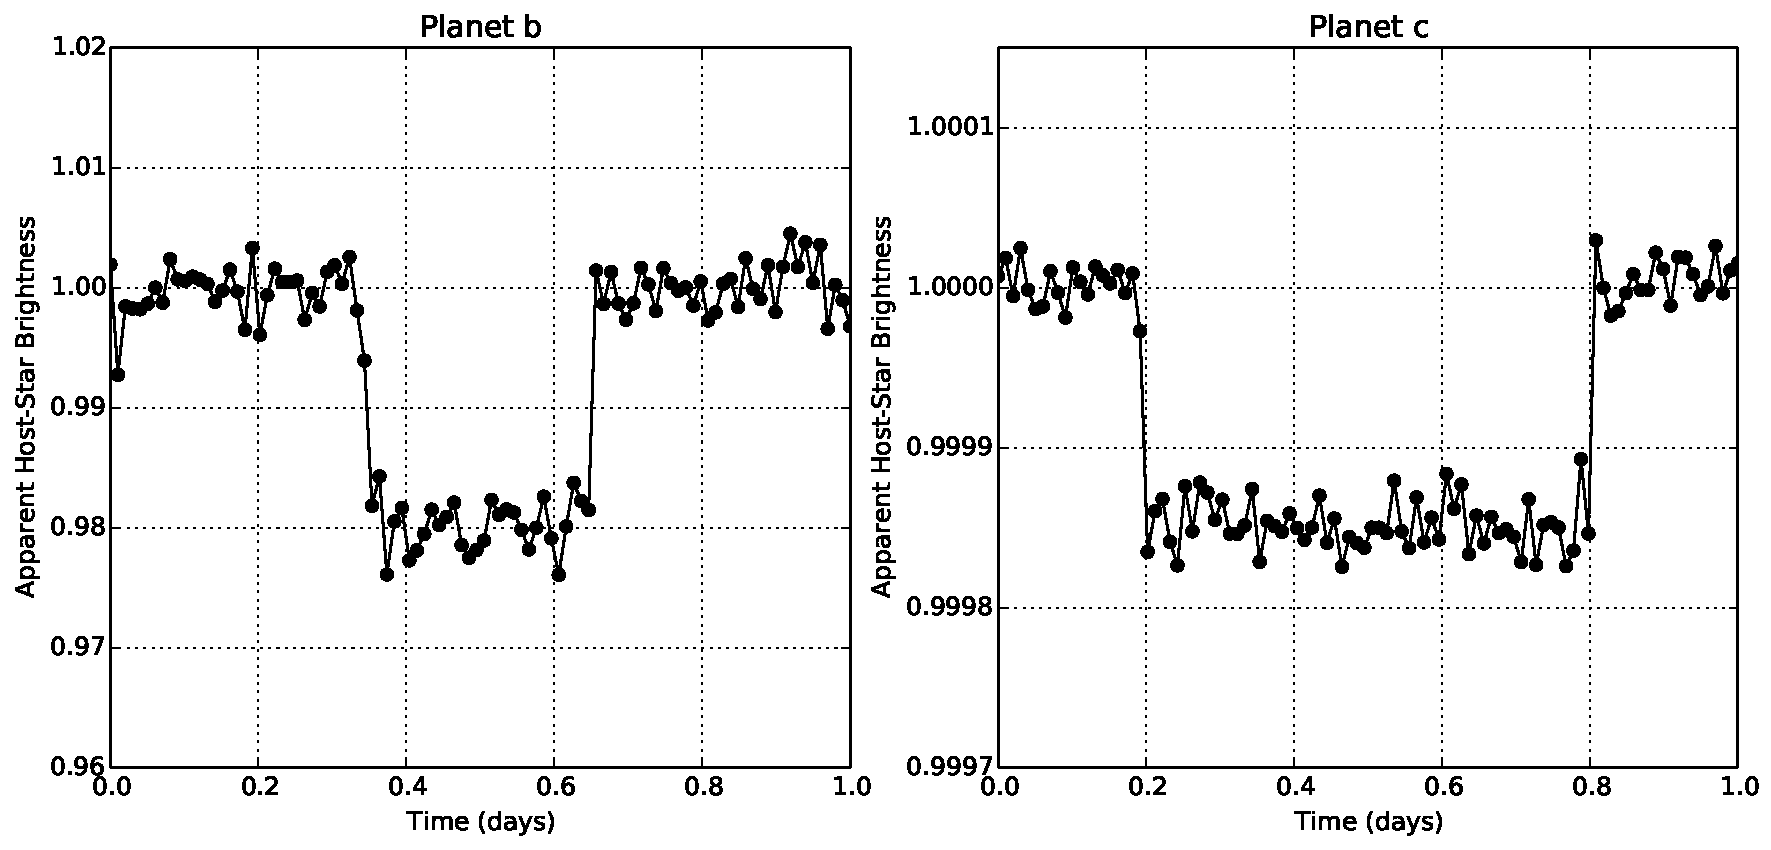
\includegraphics[scale=0.5]{plots/faketransit.pdf}
%\vspace{-5mm}
%\caption{Notice the difference in the scale of the y-axis in each plot!}
\end{figure}


\begin{table}[h!]
\centering
\begin{tabular}{|l |c |c| c| c| c|}
\hline
Planet & Period & (Change in host & Radius of & Rocky or  \\
 & (days) & star brightness)/100  &  planet  &  Gaseous? \\ \hline
b & 10 & \rule{0pt}{1.5cm} \rule{4cm}{0pt} & \rule{4cm}{0pt} & \rule{4cm}{0pt}\\ \hline
c & 300 & \rule{0pt}{1.5cm} & &\\ \hline
\end{tabular}
\end{table}

\pagebreak

\question{1} Measure the change in brightness of the star during each transit (in \%), divide that  number by 100 and record your result in the data table. 

\question{2} We want to measure the radius of each planet from the brightness data, so we need to rearrange Equation \ref{eqn:depth} like so:
\begin{equation}
\mathrm{Radius~of~the~planet} = \left( \mathrm{Radius~of~the~star} \right) \times \sqrt{\mathrm{Change~in~brightness}}
\end{equation}
If the star has a radius 109$\times$ larger than the radius of the Earth, just like our Sun, then 
\begin{equation}
\mathrm{Radius~of~the~planet~[in~Earth~radii]} = 109R_\oplus  \times \sqrt{\mathrm{Change~in~brightness}} \label{eqn:radius}
\end{equation}
Use Equation \ref{eqn:radius} and the results from Question 1 to find the radius of planets ``b'' and ``c'' that we discovered. 

\question{3} There's good reason to believe that planets with radii 1.5$\times$ larger than the Earth's are likely to be gaseous, and smaller planets are likely to be rocky. By comparing the radii of these exoplanets with the radii of planets in our solar system (Earth's radius = $1 R_\oplus$, Jupiter's radius = $11 R_\oplus$), record in the table for each planet whether you think it is gaseous like Jupiter or rocky like the Earth.


\question{4} By noticing the periods of each planet recorded for you in the table (how long it takes for the planet to complete one orbit, and for the dip in brightness pattern to repeat), as well as the radius of each planet, make an argument for which planet you'd be most likely to find life on, and why. Some potentially useful information to consider: Mercury orbits the Sun with a period of 88 days.
\vspace{4 cm}

\pagebreak
\question{5} At least one of your planets should be a rocky planet. Let's assume that the planets that you are looking at formed at the same time as our solar system 4.5 billion years ago. Do you expect this rocky planet to currently have geological activity, or would it have entered its big chill phase? Explain your reasoning.
\vspace{4 cm}


\question{6} Suppose that the planet(s) in Question 5 had an enormous, sterilizing asteroid impact 3 billion years ago that killed all lifeforms on the planet. Using your answer to Question 5, do we stand any chance of finding ancient evidence for that life on the surface today if astronauts were to land on that planet and dig around? Why or why not? ({\it Note}: travel to planets in other solar systems is not yet possible, this question is strictly hypothetical)
\vspace{4 cm}

\question{7} Using another technique, we can measure the mass of these exoplanets. An astronomer tells you that the mass of Planet b is $0.426 M_\oplus$. With the mass and radius, we have enough information to calculate the density! 

Calculate the density $D$ in units of g/cm$^3$ of the planet using the following equation: 
\begin{equation}
D = 5.515 \times \frac{M}{R^3}
\end{equation}
where $M$ is the mass of the planet in units of Earth masses and $R$ is the radius of the planet in units of Earth radii. What is this planet likely made of based on this density?

\end{document}